\documentclass[t]{beamer}
\usetheme{Warsaw}
\usepackage{array}
%\usepackage{graphicx}
\usepackage{amssymb,amsmath,mathrsfs,amsfonts}
%\usepackage[colorhighlight,display]{texpower}
%\usepackage{caption}
%\usepackage[all]{xy}
\usepackage{beamerthemesplit}
\mode<presentation>
%\usepackage{pause}
\usepackage{ulem}  % for strikethroughs
\usepackage{cancel} % for strikethroughs in math mode 
\usepackage{tikz}
\usetikzlibrary{shapes}
\usepackage{hyperref}
\hypersetup{pdfpagemode=FullScreen}
\usepackage{ifthen}
\usepackage{animate}
\usepackage{color}
\usepackage{type1cm}  % used for watermarking
\usepackage{eso-pic}  % used for watermarking


\theoremstyle{plain}
\newtheorem{prop}{Proposition}
\newtheorem{thm}[prop]{Theorem}
\newtheorem{lem}[prop]{Lemma}
\newtheorem{cor}[prop]{Corollary}
\theoremstyle{definition}
\newtheorem{dfn}{Definition}
\newtheorem{rem}[prop]{Remark}
\newtheorem{ex}{Example}[section]
%\newtheorem{note}{Note}[section]
\newtheorem{exercise}{Exercise}[section]
\newcommand{\nin}{\noindent}
\newcommand{\ds}{\displaystyle}
\renewcommand{\figurename}{Figure \arabic{figure}}



\renewcommand*\familydefault{\sfdefault} 




%%%%%%%%%%%%%%%%%%%%%%%%%%5
%%%%%%%%%%%%%%%%%%%%%%%%%%%%
%%%% some commands that have different meaning in the article/presentation modes

\newcommand{\vvfill}{\mode<presentation>{\vfill}  \mode<article>{\medskip}}   %vfill in presentation only
\newcommand{\sketchspace}{ 
\mode<article>{ \medskip\noindent{\textbf{Sketch:}} \vspace*{6cm} }
\mode<presentation>{ } 
}
\newcommand{\examplespace}{ 
\mode<article>{ \medskip\noindent{\textbf{Example:}} \vspace{6cm} }
\mode<presentation>{ } 
}
\newcommand{\artsmspace}{\mode<article>{\vspace*{2cm}} }  %small space in article mode
\newcommand{\artlargespace}{\mode<article>{\vspace*{6cm}} }  %large space in article mode

\newcommand{\dx}{\,dx}

\newcommand{\soln}{{\textbf{Solution: }}\,\,\,}
\newcommand{\disp}{\displaystyle}

\newcommand{\makedate}{\vvfill
\begin{picture}(10,10)  
\put(260,-20){\mbox{\tiny{\today}}}
\end{picture}
}

\newcommand{\pd}[2]{\dfrac{\partial#1}{\partial#2}}
\newcommand{\pD}[2]{\dfrac{\partial^2#1}{\partial#2^2}}
\newcommand{\pdd}[3]{\dfrac{\partial^2#1}{\partial#2 \partial#3}}


\normalem %stops the ulem package making all the emphs into underlines....
 
 
 
 \newcommand{\refandrev}[2]{
 \begin{small}
  \hspace{6cm}
  \begin{minipage}[r]{8cm}
  Stewart,    Chapter #1   \\
  Review:  \parbox[t]{6cm}{#2}
\end{minipage}
\end{small}
}



\newcounter{heading}
\setcounter{section}{1}
\setcounter{heading}{0}

\newcommand{\makeheading}[1]{\medskip\begin{large}\noindent\textbf{{#1}}\end{large}\smallskip}

%\newenvironment{head}[1]{\medskip\stepcounter{heading}\noindent\textbf{\hspace{0.2cm}{#1}.}}{}
\newcommand{\newhead}[1]{\medskip\stepcounter{heading}\noindent\textbf{\hspace{0.2cm}{#1}.}}


\newcommand{\pf}[1]{\noindent\textit{Proof.}\vspace*{#1 cm}}
\newcommand{\sol}[1]{\noindent\textit{Solution.}\vspace*{#1 cm}}
\newcommand{\further}[1]{\begin{small}\noindent\textit{Further reading: #1}\end{small}}
\newcommand{\exr}[1]{\begin{footnotesize}\noindent\textit{\textbf{Exercises:} Stewart #1}\end{footnotesize}}


% Sets of numbers
\newcommand{\C}{\mathbb{C}}
\newcommand{\RR}{\mathbb{R}}
\newcommand{\Z}{\mathbb{Z}}
\newcommand{\N}{\mathbb{N}}
\newcommand{\Q}{\mathbb{Q}}

% Partitions
\newcommand{\PP}{\mathcal{P}}

% Limits
\newcommand{\limm}[1]{\displaystyle \lim_{x\to #1}}

% Backslash
\newcommand{\bs}{\backslash}

% functions
\newcommand{\cosec}{\mathrm{cosec}}
\newcommand{\cosech}{\mathrm{cosech}}
\newcommand{\sech}{\mathrm{sech}}
\newcommand{\Li}{\mathrm{Li}}
\newcommand{\si}{\mathrm{Si}}
\newcommand{\erf}{\mathrm{erf}}

% Domain and Range
\newcommand{\Dom}{\mathrm{Dom}}
\newcommand{\Codom}{\mathrm{Codom}}
\newcommand{\Range}{\mathrm{Ran}}



\title{Week 2:  Limit of Functions}
\date{July 30 -- August 3, 2012}

\begin{document}

\frame{\titlepage}

\setcounter{tocdepth}{2}
\frame{\tableofcontents

\begin{flushright}
\hyperlink{tues}{\beamergotobutton{Lecture 4}}
\end{flushright} 
}

\AtBeginSection[]
{
\begin{frame}<beamer> 
\tableofcontents[currentsection]  % show TOC and highlight current section
\end{frame}
}

\section{Limits of functions at a point}
\frame
{
  \frametitle{Meaning of  limits}
  A function may or may not be defined at a particular point, but it can have a limiting value at that point.
  \pause
  
  Let us consider the function $f(x)= \ds{\frac{x^2-1}{x-1}}$.\\[3mm] \pause
  
  \begin{tabular}{|c|c|c|c|c|}\hline
  $x$ & 0.9 & 0.999 & 1.01 & 1.0001  \\ \hline
  $\ds{\frac{x^2-1}{x-1}}$ & 1.9 & 1.999 & 2.01 & 2.0001 \\ \hline
  \end{tabular}\\[3mm] \pause
  
  $f(x)$ is not defined at $x=1$, but as $x$ gets closer and closer to $1$, $f(x)$ gets closer and closer to $2$. \pause
  We say that {\em the limit of $f(x)$ as $x$ approaches to $1$, is $2$.}
  }
  
\frame
{
  \frametitle{Definition of  limits}
\begin{dfn}
Let $a$ be a real number. Suppose the function
$y=f(x)$ is defined for all $x$ near $a$ on both sides. That is, for some real numbers $b,c$ with $b<a<c$,   the intervals $(b,a)$ and $(a,c)$ are in the domain of $y=f(x)$. 
\pause
If there is a real number $L$ such that $y=f(x)$ is as close  to $L$ as desired
 by taking $x$ close ENOUGH to $a$ on both sides of $a$, then $L$ is
the {\bf limit} of $f(x)$ as $x$ approaches $a$, written
\[
\lim_{x\to a} f(x) = L.
\]
\end{dfn}
\pause
\begin{ex}
$\lim_{x\to 1}x^2 =1$.
\end{ex}
}

\frame
{
	\frametitle{Definition of  limits}
	\begin{rem}
	The limit is not affected by whether $f(a)$ is defined or what $f(a)$ is.
	\end{rem}
	\pause
	\begin{ex}
\begin{enumerate}
\item Calculate $\disp{\lim_{x\to 1}} {\dfrac{x^2-1}{x-1}}$.\pause

\nin\underline{Solution:} The domain is $(-\infty, 1)\cup (1, \infty)$. When
$x\neq 1$, ${\dfrac{x^2-1}{x-1}=\dfrac{(x+1)(x-1)}{x-1}}= x+1$.\ \pause Thus 
$\disp{
\lim_{x\to 1} (x+1) = 2.}$\pause
\item Calculate $\ds{\lim_{x\to -1}} \ds{\frac{2x+2}{x+1}}$.\pause

\nin\underline{Solution:} The domain is $(-\infty, -1)\cup (-1, \infty)$. When
$x\neq -1$, ${\dfrac{2x+2}{x+1}}= 2$. \pause 
Limit is $2$.
\end{enumerate}
\end{ex}
}

\begin{frame}
\frametitle{Limits of functions at a point}
\newhead{Examples}
\begin{enumerate}[<+->]
\addtocounter{enumi}{2}
\item if $f(x)=\begin{cases}
sin(x)&\mbox{if }x\neq 0\\
5&\mbox{if }x=0
      \end{cases}$\qquad then $\limm{0}f(x) = 0.$
\item Sometimes, the limit does not exist.\\
$\limm{0}\log_2|x|$ does not exist.

\noindent \underline{Notation:} When the limit $\ds\limm{a}f(x)$ doesn't exist because $f(x)$ becomes arbitrarily large and positive (resp. negative) as $x$ approaches $a$, we write $\ds\limm{a}f(x)=\infty$ (resp. $\ds\limm{a}f(x)=-\infty$). Thus,
\[\limm{0}\log_2|x|=-\infty.\]
\item $\ds\limm{0}\dfrac{1}{x^2}=\infty$.
\end{enumerate}

\end{frame}

\frame
{
	\frametitle{Definition of  limits}
	\begin{rem}
	{\bf One-sided limits:}

\begin{enumerate}  \item[(i)] The limit from the left:  $\disp{\lim_{x\to a^-}} f(x) =L$.
\item[(ii)] The limit from the right:  $\disp{\lim_{x\to a^+}} f(x) = L$.
\end{enumerate}
\end{rem}
\pause
\begin{ex}
$\disp{\lim_{x\to 0}} \disp{\frac{|x|}{x}}\qquad$ \underline{Solution:} The domain is $(-\infty, 0)\cup (0, \infty)$.\vspace*{-4mm}\pause
\[
\disp{\frac{|x|}{x}} = \left\{ \begin{array}{l}
+1 \qquad x>0\\[2mm]
-1 \qquad x<0.
\end{array}\right.
\]\vspace{-4mm}\pause

$\disp{\lim_{x\to 0^+}  \frac{|x|}{x}} =1$ \pause and $\disp{\lim_{x\to 0^-}  \frac{|x|}{x}} =-1$.
\end{ex}
}
\frame
{
	\frametitle{Existence of  limits}
	\begin{rem}
	The limit $\disp{\lim_{x\to a} f(x) }= L$ exists if and only if
\begin{enumerate}
\item[(i)] $\disp{\lim_{x\to a^-}} f(x)$ and $\disp{\lim_{x\to a^+}} f(x)$ exist; and \pause
\item[(ii)] $\disp{\lim_{x\to a^-}} f(x) = \disp{\lim_{x\to a^+}  f(x)}= L$.
\end{enumerate}
\end{rem}\pause

\begin{ex}
$\disp{\lim_{x\to 0}} \disp{\frac{|x|}{x}}$\pause

\nin
As $\disp{\lim_{x\to 0^+}  \frac{|x|}{x}} =1$ and $\disp{\lim_{x\to 0^-}  \frac{|x|}{x}} =-1$,
$\disp{\lim_{x\to 0}  \frac{|x|}{x}}$ doesn't exist.
\end{ex}\pause
\begin{rem}  $L\neq \pm \infty$, otherwise, the limit doesn't exist. \end{rem}
}
\frame
{
	\frametitle{Existence of  limits}
\begin{ex}
$\disp{\lim_{x\to 0}\frac{1}{x}}$\pause

\nin\underline{Solution:} The domain is $(-\infty, 0)\cup (0, \infty)$. As $x\to 0^+$, $\disp{\frac 1x}$
gets larger and larger, indicated by writing
\[
\lim_{x\to 0^+} \disp{\frac 1x}  = +\infty.
\]
As $\infty$ is not a real number, we say $\disp{\lim_{x\to 0} \frac 1x} $ does not exist.
\end{ex}\pause
\begin{rem}If $x=k$ is a vertical asymptote of $y=f(x)$, then $\disp{\lim_{x\to k}} f(x)$
doesn't exist.\end{rem}
}

\frame
{
	\frametitle{Rules for calculating limits}
\newhead{Basic limit rules} Suppose that $a\in\RR$ and that $\limm{a}f(x)$ and $\limm{a}g(x)$ exist and are finite real numbers. Then
\begin{enumerate}
\item[(i)] $\limm{a}(f(x)+g(x))=\limm{a}f(x)+\limm{a}g(x)$
\item[(ii)] $\limm{a}(f(x)-g(x))=\limm{a}f(x)-\limm{a}g(x)$
\item[(iii)] $\limm{a}f(x)g(x)=\limm{a}f(x)\limm{a}g(x)$
\item[(iv)] $\limm{a}\frac{f(x)}{g(x)}=\frac{\limm{a}f(x)}{\limm{a}g(x)}$,\,\, provided $\limm{a}g(x)\neq0$.
\end{enumerate}
A similar set of rules hold for left- and right-hand limits.
}

\frame
{
	\frametitle{Rules for calculating limits}

\newhead{Limit rule for compositions}\\ If $\limm{a}f(x)=L$ and $\limm{L}g(x)=g(L)$ then
\[\limm{a}g(f(x))=g\Big(\limm{a}f(x)\Big).\]

\smallskip

\noindent An easier way of remembering this rule will be given later.
}

\frame
{\label{tues}
	\frametitle{Recall from last class}
\newhead{Basic limit rules} Suppose that $a\in\RR$ and that $\limm{a}f(x)$ and $\limm{a}g(x)$ exist and are finite real numbers. Then
\begin{enumerate}
\item[(i)] $\limm{a}(f(x)+g(x))=\limm{a}f(x)+\limm{a}g(x)$
\item[(ii)] $\limm{a}(f(x)-g(x))=\limm{a}f(x)-\limm{a}g(x)$
\item[(iii)] $\limm{a}f(x)g(x)=\limm{a}f(x)\limm{a}g(x)$
\item[(iv)] $\limm{a}\frac{f(x)}{g(x)}=\frac{\limm{a}f(x)}{\limm{a}g(x)}$,\,\, provided $\limm{a}g(x)\neq0$.
\end{enumerate}
A similar set of rules hold for left- and right-hand limits.
}

\frame
{
	\frametitle{Rules for calculating limits}


\newhead{Example}

\vspace*{-3mm}\begin{center}
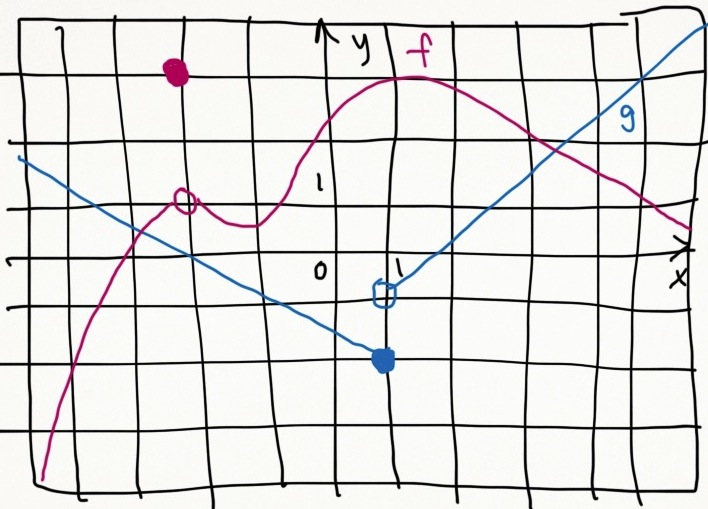
\includegraphics[width=45mm]{Ch1limitsfigure.jpg}
\end{center}  
  
  \noindent Use the limit laws and the graphs of $f$ and $g$ in the above figure to evaluate the following limits, if they exist.
  \begin{enumerate}[<+->]
  \item[(a)] $\limm{-2}[f(x) + 5g(x)]$
  \item[(b)] $\limm{1}[f(x)g(x)]$
  \item[(c)] $\limm{2}\frac{f(x)}{g(x)}$
  \end{enumerate}

}


\section{Limits at infinity}
\begin{frame}
\frametitle{Limits at infinity}
\noindent There are many situations where it is desirable to know what the eventual state of a system will be.

\

\noindent\begin{small}
 \textit{\bf Example:} Suppose that an initially unpolluted lake containing 1 gigalitre ($10^{9}$ litres) of water has a river flowing through it at a rate of 1 megalitre ($10^{6}$ litres) per day. A factory is built next to the lake and discharges ten thousand ($10^{4}$) litres of pollution per day. Environmental authorities want to know what the eventual impact of the pollution will be.
 By making some simple assumptions, it can be shown that the amount $P(t)$ of pollution (in litres) in the lake after $t$ days of the factory's operation is given by
\begin{equation}\label{eq:pollution model}
P(t)=\frac{10^9}{101}\big(1-e^{-101t/10^5}\big).
\end{equation}
To see whether the pollution in the lake eventually stabilizes, and what the level of pollution will be, one studies the behavior of $P(t)$ as $t\to\infty$.
\end{small}
\end{frame}

\begin{frame}
\frametitle{Calculating limits at infinity}
\newhead{Definition (imprecise)}

\noindent if $f$ is a function defined on an interval $(a, \infty)$, or $(-\infty, \infty)$, then
\[ \lim_{x\rightarrow \infty} f(x) = L\]
means that the values of $f(x)$ can be made arbitrarily close to $L$ by taking $x$ sufficiently large.

Sometimes we also write
\[ f(x) \longrightarrow L \qquad \text{as} \qquad x \longrightarrow \infty\]


\end{frame}

\begin{frame}

\uncover<+->{\newhead{Examples} True or False?}
\begin{enumerate}[<+->]
\item[(a)] $\limm{\infty} x = \infty$
\item[(b)] $\limm{\infty} x^{2} = \infty$
\item[(c)] $\limm{\infty} x^{3} = \infty$
\item[(d)] $\limm{\infty} x^{-1} = \infty$
\item[(e)] $\limm{\infty} sin(x) =  0$
\item[(f)] $\limm{\infty} e^{x} = \infty$
\item[(g)] $\limm{\infty} \sqrt{x} = 2$
\item[(h)] $\limm{\infty} ln(x) = 100$
\end{enumerate}
\end{frame}

\begin{frame}
\uncover<+->{\noindent We have a similar definition for the limit as $x$ goes to $-\infty$:

\noindent Let $f$ be a function defined on some interval $(-\infty, a)$ or $(-\infty, \infty)$.  Then 
\[\lim_{x\rightarrow -\infty}f(x) = L\]
means that the values of $f(x)$ can be made arbitrarily close to $L$ by taking $x$ sufficiently large and negative.}

\uncover<+->{\vspace*{.1cm}
\newhead{Question} What is the value of $\limm{-\infty} e^{x}$?}

\uncover<+->{\vspace*{.1cm}

\noindent The line $y=L$ is called a \emph{horizontal asymptote} of the curve $y = f(x)$ if either 
\[ \lim_{x\rightarrow \infty}f(x) = L \qquad \text{or} \qquad \lim_{x\rightarrow -\infty}f(x) = L.\]}
\end{frame}

\begin{frame}
\newhead{Basic rules} Suppose that $\limm{\infty}f(x)$ and $\limm{\infty}g(x)$ exist and are \underline{finite} real numbers. Then
\begin{enumerate}[<+->]
\item[(i)] $\limm{\infty}[f(x)+g(x)]=\limm{\infty}f(x)+\limm{\infty}g(x)$
\item[(ii)] $\limm{\infty}[f(x)-g(x)]=\limm{\infty}f(x)-\limm{\infty}g(x)$
\item[(iii)] $\limm{\infty}[f(x)g(x)]=[\limm{\infty}f(x)][\limm{\infty}g(x)]$
\item[(iv)] $\limm{\infty}\frac{f(x)}{g(x)}=\frac{\limm{\infty}f(x)}{\limm{\infty}g(x)}$, provided $\limm{\infty}g(x)\neq0$.
\item[(v)] if $\limm{\infty}f(x) = \infty$, then $\limm{\infty}\frac{1}{f(x)}= 0$.
\end{enumerate}

\vspace*{.2cm}

\uncover<+->{\newhead{Examples}}
\begin{enumerate}[<+->]
\item[(a)]$\limm{\infty}(\frac{1}{x} + 1 - e^{-2x})$
\item[(b)]$\limm{-\infty}(\frac{3}{x} + 1 - cos(x))$ 
\end{enumerate}
\end{frame}

\begin{frame}[title=The squeeze theorem]
\noindent Not all limits can be evaluated using the direct substitution property and the above rules.\pause


\newhead{The squeeze theorem} Suppose that $f(x)\leq g(x)\leq h(x)$ when $x$ is near $a$ (except possibly at $a$)
and
\[\limm{a}f(x)=\limm{a}h(x)=L.\]
Then
\[\limm{a}g(x)=L.\]\pause

\noindent (Similar versions of the squeeze theorem exist for left- and right-hand limits.)\pause

\newhead{Example} Find $\limm{0}x^2\sin(1/x)$.

\end{frame}

\begin{frame}[title=The squeeze theorem]
\newhead{The squeeze theorem for limits at infinity} Suppose that $f$, $g$ and $h$ are all defined on the interval $(b,\infty)$, where $b\in\RR$. If
\[f(x)\leq g(x)\leq h(x)\qquad\forall x\in(b,\infty)\]
and
\[\limm{\infty}f(x)=\limm{\infty}h(x)=L\]
then
\[\limm{\infty}g(x)=L.\]\pause

\vspace*{.2cm}

\newhead{Example} Use the squeeze theorem to find $\limm{\infty}\frac{\sin x}{x}$.

\end{frame}

\begin{frame}
\newhead{Indeterminate forms}

\uncover<+->{\noindent Limits of the type
\[\limm{\infty}\frac{f(x)}{g(x)}\]
where $f(x)\to\infty$ and $g(x)\to\infty$ as $x\to\infty$ are said to be limits of the form $\frac{\infty}{\infty}$.}
\uncover<+->{While the following limits have the form $\frac{\infty}{\infty}$, each displays very different limiting behavior as $x\to\infty$:}
\begin{itemize}[<+->]
\item $\qquad$ $\limm{\infty}\frac{x}{x}$
\item $\qquad$ $\limm{\infty}\frac{x}{x^{2}}$
\item $\qquad$ $\limm{\infty}\frac{x^{3}}{x}$
\item $\qquad$ $\limm{\infty}\frac{e^{x}}{x}$ $\qquad$ (deal with this more later)
\end{itemize}

\end{frame}



\end{document}